\documentclass{standalone}

\usepackage{tikz}
\usetikzlibrary{angles,quotes}
\usepackage{amsmath,amssymb,amsfonts}

\usepackage{pgfplots}
\definecolor{darkgreen}{rgb}{0.0, 0.42, 0.24}
\definecolor{amethyst}{rgb}{0.6, 0.4, 0.8}

\pgfplotsset{compat=newest}
\pgfplotsset{every axis/.append style={
                     tick label style={font=\footnotesize},
                 }}


\begin{document}
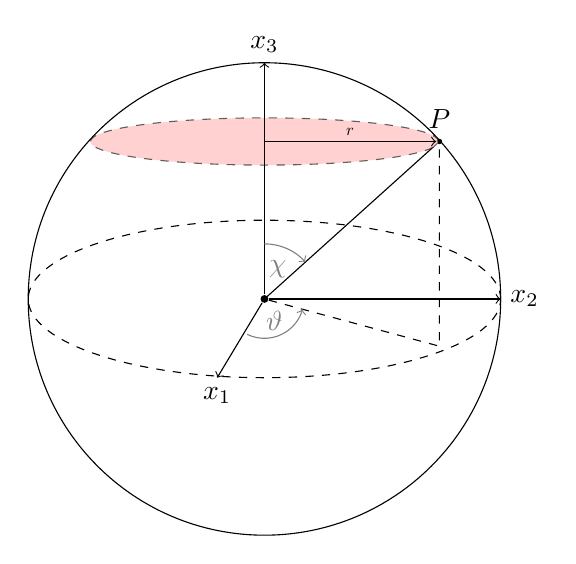
\begin{tikzpicture}

    % Define radius
    \def\r{3}

    % Bloch vector
    \draw (0,0) node[circle,fill,inner sep=1] (orig) {} -- (\r/1.35,\r/1.5) node[circle,fill,inner sep=0.7,label=above:$P$] (a) {};
    \draw[dashed] (orig) -- (\r/1.35,-\r/5) node (phi) {} -- (a);
\draw (0,2) node (p){};
\draw (-0.13,2) node(cenz){};
    % Sphere
    \draw (orig) circle (\r);
    \draw[dashed] (orig) ellipse (\r{} and \r/3);
    \draw[dashed, fill=red!30,opacity=0.6] (p) ellipse (2.21 and 0.3);
 
    % Axes
    \draw[->] (orig) -- ++(-\r/5,-\r/3) node[below] (x1) {$x_1$};
    \draw[->] (orig) -- ++(\r,0) node[right] (x2) {$x_2$};
    \draw[->] (orig) -- ++(0,\r) node[above] (x3) {$x_3$};

    \draw[->] (cenz)--(a) node[above,midway,scale=0.6]{$r$};

    %Angles
    \pic [draw=gray,text=gray,->,"$\vartheta$"] {angle = x1--orig--phi};
    \pic [draw=gray,text=gray,<-,"$\chi$",scale=1.4] {angle = a--orig--x3};

\end{tikzpicture}
\end{document}